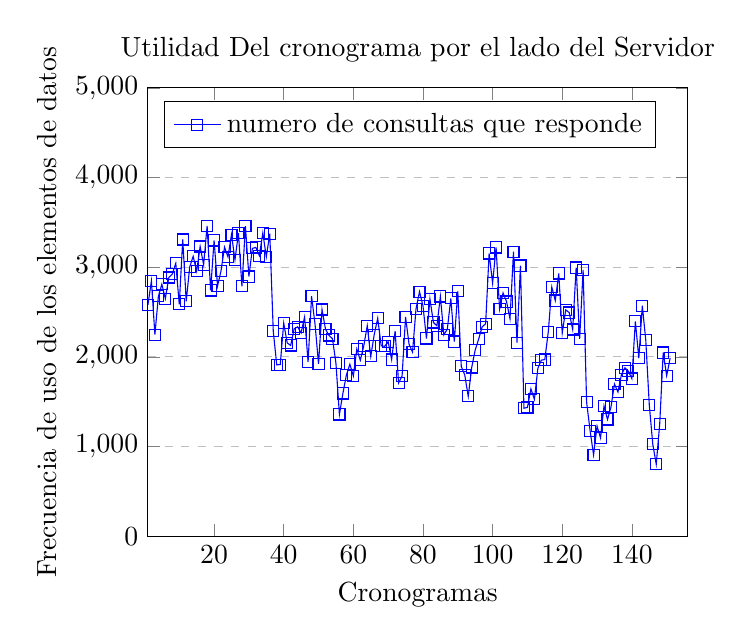
\begin{tikzpicture}
\begin{axis}[
    title={Utilidad Del cronograma por el lado del Servidor},
    xlabel={Cronogramas},
    ylabel={Frecuencia de uso de los elementos de datos},
    xmin=1, xmax=156,
    ymin=0, ymax=5000,
    xtick={},
    ytick={},
    legend pos=north west,
    ymajorgrids=true,
    grid style=dashed,
]

\addplot[
    color=blue,
    mark=square,
    ]
    coordinates {
%UTILIDAD TOTAL
(1,2578)
(2,2848)
(3,2248)
(4,2675)
(5,2810)
(6,2649)
(7,2885)
(8,2923)
(9,3044)
(10,2585)
(11,3309)
(12,2620)
(13,3003)
(14,3121)
(15,2956)
(16,3231)
(17,3028)
(18,3460)
(19,2741)
(20,3298)
(21,2791)
(22,2960)
(23,3224)
(24,3115)
(25,3363)
(26,3083)
(27,3379)
(28,2787)
(29,3459)
(30,2896)
(31,3210)
(32,3220)
(33,3129)
(34,3382)
(35,3116)
(36,3373)
(37,2285)
(38,1912)
(39,1913)
(40,2376)
(41,2156)
(42,2127)
(43,2313)
(44,2335)
(45,2267)
(46,2444)
(47,1942)
(48,2676)
(49,2365)
(50,1921)
(51,2528)
(52,2309)
(53,2239)
(54,2203)
(55,1930)
(56,1358)
(57,1592)
(58,1797)
(59,1918)
(60,1787)
(61,2088)
(62,1962)
(63,2123)
(64,2347)
(65,2005)
(66,2248)
(67,2431)
(68,2123)
(69,2117)
(70,2169)
(71,1970)
(72,2287)
(73,1708)
(74,1786)
(75,2445)
(76,2142)
(77,2053)
(78,2535)
(79,2727)
(80,2570)
(81,2205)
(82,2646)
(83,2384)
(84,2346)
(85,2674)
(86,2245)
(87,2310)
(88,2652)
(89,2171)
(90,2730)
(91,1894)
(92,1798)
(93,1559)
(94,1882)
(95,2076)
(96,2199)
(97,2335)
(98,2369)
(99,3153)
(100,2823)
(101,3220)
(102,2533)
(103,2713)
(104,2617)
(105,2425)
(106,3172)
(107,2158)
(108,3018)
(109,1427)
(110,1436)
(111,1643)
(112,1527)
(113,1872)
(114,1963)
(115,1970)
(116,2281)
(117,2779)
(118,2628)
(119,2930)
(120,2266)
(121,2524)
(122,2494)
(123,2305)
(124,2996)
(125,2201)
(126,2969)
(127,1496)
(128,1177)
(129,907)
(130,1227)
(131,1096)
(132,1453)
(133,1302)
(134,1440)
(135,1697)
(136,1608)
(137,1800)
(138,1878)
(139,1840)
(140,1758)
(141,2396)
(142,1985)
(143,2571)
(144,2184)
(145,1466)
(146,1028)
(147,802)
(148,1252)
(149,2048)
(150,1790)
(151,1987)
    };
    \legend{numero de consultas que responde}

\end{axis}
\end{tikzpicture}

